\newpage
\section{Descrizione architettura}
\subsection{Metodo e formalismo di specifica}
Le scelte progettuali di \glossaryItem{MaaS} sono state fortemente influenzate dallo stack tecnologico usato. \\
L'intera applicazione è stata progettata per essere scritta con un unico linguaggio: TypeScript. Questo linguaggio è un \textit{superset} di \glossaryItem{JavaScript} che viene compilato in normale \glossaryItem{JavaScript}. La scelta è ricaduta su TypeScript perchè rende più leggibile ed intuitivo il codice prodotto, oltre a permettere i controlli statici che in \glossaryItem{JavaScript} non sono presenti.
La progettazione del backend è stata influenzata pesantemente anche dal \glossaryItem{framework} scelto: ExpressJS. Questo \glossaryItem{framework} è basato su \glossaryItem{Node.js} e permette di creare velocemente ed intuitivamente dei webserver per l'esposizione di \glossaryItem{API} \glossaryItem{REST}. \\
Per esporre l'architettura dell'applicazione si procederà con approccio \glossaryItem{top-down}, partendo cioè da una visione generale delle componenti che distinguono il sistema, per poi analizzare in dettaglio la conformazione di tali componenti. Per descrivere in maniera formale l'architettura verranno impiegati lo standard \glossaryItem{UML} 2.0 per i \glossaryItem{diagrammi} dei \glossaryItem{package} e delle classi e lo standard \glossaryItem{UML} 2.4 per i \glossaryItem{diagrammi} di attività e sequenza. \\

Viene fatto uso inoltre di un codice a colori per distinguere la provenienza dei \glossaryItem{moduli} dell'applicazione. In particolare:
\begin{itemize}
\item in colore \textbf{giallo} i \glossaryItem{moduli} da implementare;
\item in colore \textbf{verde} vengono proposti i \glossaryItem{moduli}/librerie importati dal \textit{Core} delle tecnologie utilizzate e da terze parti.
\end{itemize}

I \glossaryItem{diagrammi} delle classi che permettono di mostrare l'architettura generale del sistema vengono affiancati anche dai \glossaryItem{diagrammi} di sequenza e attività, che permettono di definire le interazioni tra le componenti, senza preoccuparsi della loro classificazione. In questo modo è possibile esprimere alcuni meccanismi tipici di un'applicazione \glossaryItem{REST}-like, come il modo in cui agiscono i \glossaryItem{middleware}. 

\subsection{Architettura generale}
L'architettura del \glossaryItem{progetto} si divide in una componente Client, rappresentata da un'applicazione frontend accessibile da un browser, e in una componente WebServer, nella quale risiede il backend. 

\subsection{Conformazione generale dell'architettura}
L'architettura generale di \glossaryItem{MaaS} si può dividere in 3 macrocomponenti:
\begin{itemize}
\item \textbf{Server \glossaryItem{REST}}; 
\item \textbf{Client}; 
\item \textbf{Editor}.
\end{itemize}
\begin{figure}[h]
\centering
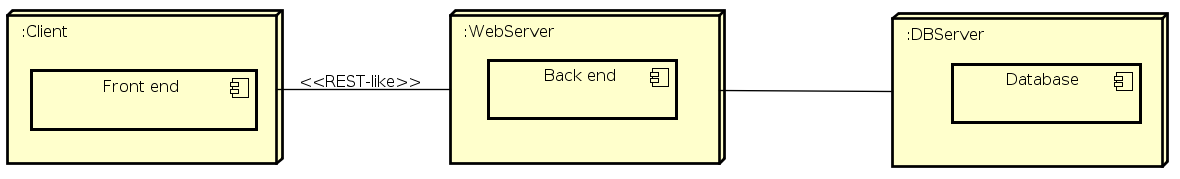
\includegraphics[width=0.8\textwidth]{res/sections/GeneralArchitecture.png}
\caption{Diagramma di \glossaryItem{deployment} per l'architettura}
\end{figure}
L'architettura proposta segue il \glossaryItem{Design Pattern} MVC. In particolare i ruoli di Model e Controller verranno implementati a livello di server, mentre il ruolo di View viene affidato al frontend. L'interfaccia tra le due componenti verrà gestita grazie ad un set di \glossaryItem{API} disposto dal server \glossaryItem{REST}: in questo modo si garantisce una totale indipendenza tra frontend e backend e sono possibili sviluppi futuri anche in altre piattaforme (ad esempio in app mobile) senza dover creare dei sistemi di integrazione ad-hoc. \\
Le tre macrocomponenti verranno descritte in dettaglio in seguito su questo documento.
\subsection{Interfaccia REST-like}
Il backend si basa su uno stile \glossaryItem{REST}-like, ovvero con le seguenti caratteristiche:
\begin{itemize}
\item stato dell'applicazione e funzionalità divisi in risorse web;
\item ogni risorsa è unica e indirizzabile attraverso un \glossaryItem{URI} (\textbf{U}niform \textbf{R}esource \textbf{I}dentifier);
\item tutte le risorse sono condivise come interfaccia uniforme per il trasferimento di stato tra client e risorse. Questo trasferimento consiste in:
\begin{itemize}
\item un insieme vincolato di operazioni ben definite;
\item un insieme vincolato di contenuti, opzionalmente supportato da codice a richiesta;
\item un protocollo:
\begin{itemize}
\item client-server;
\item privo di stato;
\item memorizzabile in cache;
\item a livelli.
\end{itemize}
\end{itemize}
\end{itemize}
REST utilizza il concetto di risorsa (aggregato di dati con un nome, l'URI, e una rappresentazione interna), sulla quale è possibile invocare operazioni CRUD (\textbf{C}reate, \textbf{R}ead, \textbf{U}pdate, \textbf{D}elete) con la seguente corrispondenza:
\begin{table}[H]
\centering
\label{CRUD}
\begin{tabular}{| >{\centering}p{3cm} | >{\centering}p{5cm} | >{\centering}p{6cm} |}
\hline
\textbf{Risorsa} & \textbf{URI della \glossaryItem{collection}} \newline es. http://maas.com/users & \textbf{URI della risorsa} \newline es. http://maas.com/users/10 \tabularnewline \hline
\textbf{GET} & Fornisce informazioni sui membri della \glossaryItem{collection}. & Fornisce una rappresentazione dell'elemento della \glossaryItem{collection} indicato. \tabularnewline \hline
\textbf{PUT} & Non usata. & Sostituisce una rappresentazione dell'elemento della \glossaryItem{collection} indicato. Se non esiste lo crea.  \tabularnewline \hline
\textbf{POST} & Crea un nuovo elemento della \glossaryItem{collection}. La \glossaryItem{URI} del nuovo elemento è generata automaticamente. & Non usato. \tabularnewline \hline
\textbf{DELETE} & Non usata. & Cancella l'elemento della \glossaryItem{collection} indicato. \tabularnewline \hline
\end{tabular}
\caption{Tabella delle operazioni CRUD}
\end{table}
Per la rappresentazione dei dati si è scelto di utilizzare \glossaryItem{JSON} perché si integra molto bene con i \glossaryItem{framework} utilizzati e con il linguaggio \glossaryItem{JavaScript}. Questo non è vero per \glossaryItem{XML} (e\textbf{X}tensible \textbf{M}arkup \textbf{L}anguage) o \glossaryItem{CSV} (\textbf{C}omma \textbf{S}eparated \textbf{V}alues), che richiederebbero librerie specifiche. Inoltre \glossaryItem{JSON} è molto meno verboso e molto più flessibile di \glossaryItem{XML}, e si adatta molto bene al dominio dell'applicazione.
